\documentclass[a4paper,12pt,twoside]{article}

% Pacotes de compilação
    % Formatação
\usepackage[utf8]{inputenc} % não precisa ficar colocando \c para caracteres especiais
\usepackage{indentfirst}
\usepackage{caption}
\usepackage{subcaption}
\usepackage{array}
    % Imagens
\usepackage{graphicx}
\usepackage{float}
    % Math
\usepackage{textcomp}
\usepackage{siunitx}
\usepackage{amsmath}
\usepackage{amssymb}

% Table centering -> array package
\newcolumntype{P}[1]{>{\centering\arraybackslash}p{#1}}
\newcolumntype{M}[1]{>{\centering\arraybackslash}m{#1}}

%Bibliografia
\usepackage{natbib}

%Idioma
\usepackage[portuguese]{babel}

% Pacotes de citações
    % Paginas com as citações na bibl
% \usepackage[brazilian,hyperpageref]{backref}
    % Citações padrão ABNT
% \usepackage[alf]{abntex2cite}

% Configurações da página
\setlength{\paperwidth}{21cm}          % Largura da página
\setlength{\paperheight}{29,7cm}       % Altura da página
\setlength{\textwidth}{15.5cm}         % Largura do texto
\setlength{\textheight}{24.6cm}        % Altura do texto
\setlength{\topmargin}{-1.0cm}         % Margem superior da página = 1 polegada + valor atribuição.
                                       % \setlenght{\topmargin}{0cm} dá 2.54cm de margem superior.
\setlength{\oddsidemargin}{0.46cm}     % Margem esquerda = 1 polegada + valor
\setlength{\evensidemargin}{0.46cm} 

% ================== DOCUMENTO ====================== %

\begin{document}

\thispagestyle{empty}

\begin{figure}
  \centering
  
\includegraphics[scale=0.4]{images/logo-usp-ifsc.png}
  \vspace*{-0.3cm}
\end{figure}

\begin{center}
{\large \rm \textbf {LABORATÓRIO DE FÍSICA II} \linebreak}
\end{center}

\baselineskip 30pt

\vspace*{0.3cm}

\begin{center}
{\LARGE \bfseries Prática V - Processos Térmicos em Gases}
\end{center}

\vspace*{1cm}

\setcounter{footnote}{1}

\renewcommand{\thefootnote}{\fnsymbol{footnote}}
\begin{center}
{
    \sc  André Zanardi Creppe - 11802972 \\
    \sc  Gabriel de Oliveira Maia - 11819790 \\
    \sc  Vitor Malosso Micheletti - 10738291 \\
}
\vspace*{0.5cm}

\center{\rm  Professores:} 
\vspace*{-.5cm}
\center{\sc Emanuel Alves de Lima Henn \\ Leonardo De Boni}
\end{center}

% \setcounter{footnote}{1}

\baselineskip 17pt

\vspace*{1.5cm}
\begin{center}
{{\bf Novembro de 2020}}
\end{center}

\vspace*{.05cm}

\renewcommand{\thefootnote}{\arabic{footnote}}

\setcounter{footnote}{1}

\pagebreak

\baselineskip 19pt

\tableofcontents
\newpage
\section{Objetivos}



\newpage
\section{Materiais e métodos}

% =============== EXPERIMENTO 1 ===================== %

\subsection{Determinação do Momento de Inércia de um disco}

Uma das montagens experimentais que utilizaremos nessa prática é a do Disco de Maxwell. Ela consiste num disco que está preso a um eixo e que possui dois fios de barbante amarrados nas extremidades. Isso permite que ele seja solto de uma altura qualquer e acelere para baixo ganhando energia cinética de translação e rotação, possibilitando fazer uma análise quantitativa desses dois fenômenos. 

\begin{figure}[H]
  \centering
  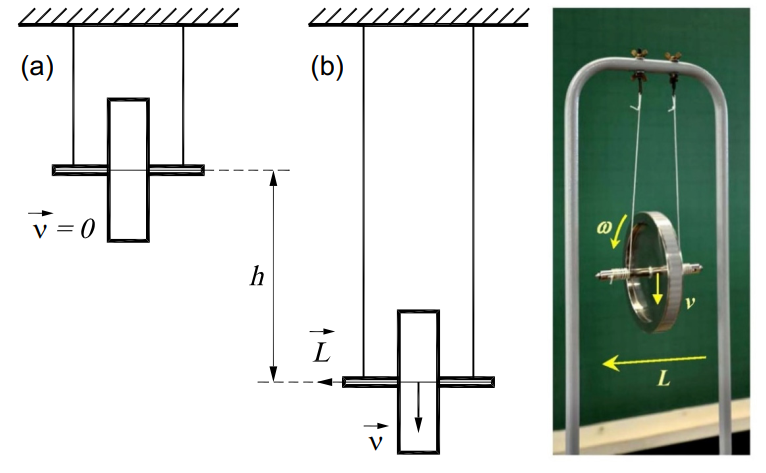
\includegraphics[scale=0.5]{images/setup-maxwell.png}
  \caption{Montagem experimental do Disco de Maxwell}
\end{figure}

Num primeiro momento, desmontaremos o disco e utilizaremos as medidas de cara componente dele para determinar o seu momento de inércia, que será a soma dos momentos de cada componente. Como ele é feito de basicamente um cilindro inteiro (eixo) e 2 cilindros com furo (anel externo + disco), nós sabemos que o momento de inércia total será a soma dos momentos de inércia de cada peça:

\[I_T = I_E + I_A + I_D\]

Com a incerteza sendo a simples soma das incertezas de cada componente:

\[\Delta I_T = \Delta I_E + \Delta I_A + \Delta I_D\]

E cada um desses componentes pode ser calculado a partir dessas 2 fórmulas para cilindros inteiros (CI) e cilindros com furo (CF):

\[I_{CI} = \frac{1}{2}MR^2\]
\[I_{CF} = \frac{1}{2}M(R^2 + R_1^2)\]

Propagando as incertezas desses nesses dois casos teremos:

\[\Delta I_{CI} = \frac{1}{2} \left( \Delta M \cdot R^2 + 2 \cdot R \cdot \Delta R \cdot M \right)\]
\[\Delta I_{CF} = \frac{1}{2} 
    \left[ 
        \Delta M \cdot (R^2 + R_1^2) + 
        \left( 2 \cdot R \cdot \Delta R + 2 \cdot R_1 \cdot \Delta R_1 \right) \cdot M
    \right]
\]

Agora, vamos calcular por meio da queda o momento de inércia do disco. Para isso, primeiro precisaremos determinar uma altura \textit{h} para ser o nosso referencial de energia potencial gravitacional. Podemos utilizar o fio totalmente estendido como o ponto mais baixo, e a partir daí enrolar da forma que desejar.\\

Após escolher tal altura será feito 3 medições do tempo de queda de acordo com o esquema (a) e (b) da figura anterior. Essas medições serão feitas com um cronometro de precisão. Com 3 valores iniciais e finais para \textit{$t_b$} - tempo para chegar no estado (b) - encontrados, faremos a subtração deles e depois uma média média aritmética para achar $\overline{t}_b$, e a sua incerteza pelo desvio padrão dessas medidas:

\[\overline{t}_b = \frac{t_{b1} + t_{b2} + t_{b3}}{3}\]

\[\Delta \overline{t}_b = \sqrt{\frac{\sum_{i=1}^{3} (t_i - \overline{t})^2}{3}}\]

Com $\overline{t}_b$ depois poderemos calcular o valor do momento de inércia \textit{I} do disco em estudo e utilizando a seguintes fórmula que foi deduzida na apostila do curso e nos vídeos:

\[I = \left( \frac{g \overline{t}_b^2}{2h} - 1 \right) mr^2\]

E a incerteza \textit{$\Delta$I} dessa medida será dada por:

\[\Delta I = \Delta P \cdot Q + \Delta Q \cdot P\]

Onde $\Delta$P é a propagação do que está dentro dos parênteses, e $\Delta$Q o termo do lado de fora.

\[
    \Delta P = \frac{g}{2} 
    \left( 
        \frac
        {\overline{t}_b^2 \cdot \Delta H + 2 \cdot \overline{t}_b \cdot \Delta \overline{t}_b \cdot h}
        {h^2} 
    \right)
\]
\[\Delta Q = 2mr \Delta r + \Delta m r^2\]

% =============== EXPERIMENTO 2 ===================== %

\subsection{Choques Rotacionais}

O segundo experimento consiste em analisar o choque rotacional de um sistema formado por duas peças cilíndricas rotacionando em torno do mesmo eixo de rotação, sem atrito. Em determinado instante de tempo, a peça que está acima (peça 2) é solta e cai sobre a peça que está abaixo (peça 1) no sistema. Então, devido ao atrito entre as superfícies das duas peças, o conjunto passa a girar a uma velocidade angular comum. O sistema pode ser representado com base na Figura 2.1 abaixo:

\begin{figure}[H]
  \centering
  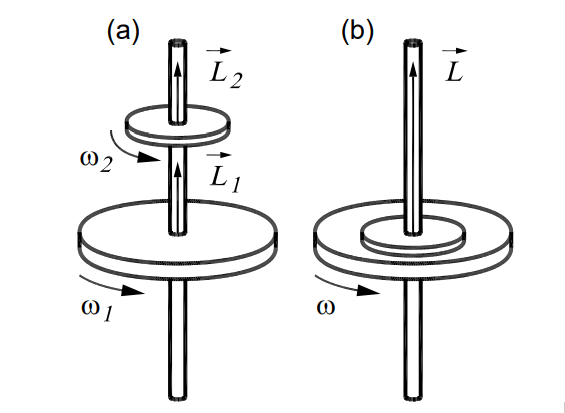
\includegraphics[scale=0.8]{images/choque_rotacional.png}
  \caption{Sistema formado por duas peças cilíndricas que giram em torno do mesmo eixo de rotação com velocidades angulares distintas 1 e 2 (a). Em certo instante de tempo, as peças formam um conjunto que passa a girar a uma mesma velocidade angular (b).}
\end{figure}

Com base na Figura 2.1, pode-se caracterizar algumas grandezas que foram utilizadas durante o experimento:

\begin{table}[H]
    \centering
    % \begin{tabular}{ |M{2cm}||M{8cm}| }
    \begin{tabular}{ |c||c| }
        \hline
        \textbf{Símbolo} & \textbf{Grandeza}\\
        \hline
        $\omega _1$     & Velocidade Angular inicial da Peça 1\\
        $\omega _2$     & Velocidade Angular inicial da Peça 2\\
        $\omega $       & Velocidade Angular final do conjunto\\
        \hline
        L$_1$   & Momentum Angular inicial da Peça 1\\
        L$_2$   & Momentum Angular inicial da Peça 2\\
        L       & Momentum Angular final do conjunto\\
        \hline
    \end{tabular}
    \caption{Legenda das grandezas}
\end{table}

As peças são caracterizadas como um disco maciço com eixo central (mesmo disco utilizado no experimento anterior com a roda de Maxwell e referido como peça 1) e um cilindro oco (peça 2). Baseado na imagem, também é possível visualizar a direção e sentido dos vetores envolvidos na rotação das peças.\\

Então, inicialmente a peça 1 é colocada em rotação e a peça 2 na parte superior é mantida em repouso e segurada por uma porca (S) para não cair. Ao afrouxar a porca, a peça 2 cai e colide com a peça 1. As velocidades de rotação inicial e final foram medidas com um tacômetro óptico, que conta as franjas na lateral da peça 1.

\begin{figure}[H]
  \centering
  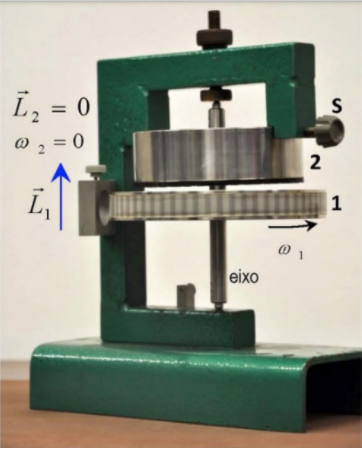
\includegraphics[scale=0.8]{images/experimento_choque.png}
  \caption{Montagem experimental real, com seus respectivos elementos, para analisar o choque rotacional entre duas peças cilíndricas.}
\end{figure}

Com base nas características geométricas e na massa do cilindro oco (Peça 2), foi determinado o Momento de Inércia ($I_2$) com sua respectiva incerteza experimental. As medidas foram determinadas com auxílio de um paquímetro e de uma balança digital para o raio e a massa da peça, respectivamente.\\

Após isso, foi feito uma análise dos resultados representados no segundo vídeo (minuto 31:50 - 36:20) que mostra uma medida quantitativa da diminuição da velocidade angular de rotação da peça 1 devido a torques dissipativos. Com essa análise e o Momento de Inércia da peça 1 ($I_1$) calculado no experimento anterior, foi construído um gráfico da energia de rotação da roda com função do tempo. E então, determinou-se a energia média perdida pelo sistema em um ciclo de oscilação.\\

Para esse experimento, foram realizados três choques rotacionais e em cada um deles foi determinado a velocidade angular imediatamente antes e depois da colisão.Nesse momento, os dados foram obtidos a partir de um software que calcula a velocidade angular com base em um sistema de infravermelho e arduino instalados previamente.O software fornece a velocidade angular em diversos momento e devemos utilizar os pontos que correspondem ao momento imediatamente antes e depois da colisão.\\

Assumindo que houve conservação do momentum angular durante a colisão, determinou-se o Momento de Inércia $I_1$ da peça 1 utilizando a seguinte equação:

\[ \omega = \frac{I_1 \omega_1+I_2 \omega_2}{I_1+I_2} \]

Por fim, calculou-se as energias cinéticas rotacionais, antes e depois da colisão, e sua variação relativa, para, então, verificar se houve ou não conservação da energia cinética. Os resultados obtidos foram comparados ao experimento anterior da Roda de Maxwell para se discutir a confiabilidade de cada método.


% =============== EXPERIMENTO 3 ===================== %

\subsection{Conservação do Momento Angular}

aaaaaaaa

% =============== EXPERIMENTO 4 ===================== %

\subsection{Precessão do Giroscópio}

O último experimento sobre esse tópico que vamos realizar é sobre giroscópios, mais precisamente o fenômeno da precessão que eles realizam, que consiste no movimento circular realizado em torno de um ponto de pivô por um objeto que gira, como pode ser visto nas figuras abaixo:

\begin{figure}[H]
  \centering
    \begin{subfigure}[b]{0.48\textwidth}
        \centering
        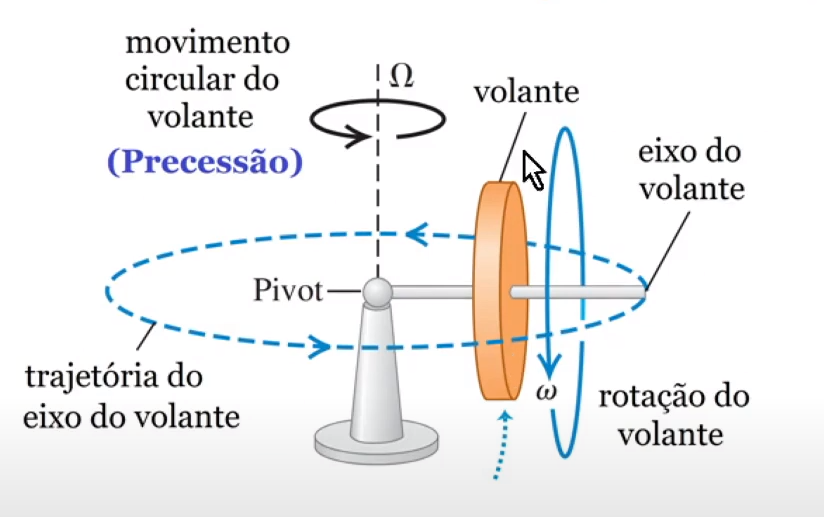
\includegraphics[width=\textwidth]{images/movimento-giroscopio.png}
        \caption{Diagrama do movimento de precessão de um giroscópio}
    \end{subfigure}
    \hfill
    \begin{subfigure}[b]{0.48\textwidth}
        \centering
        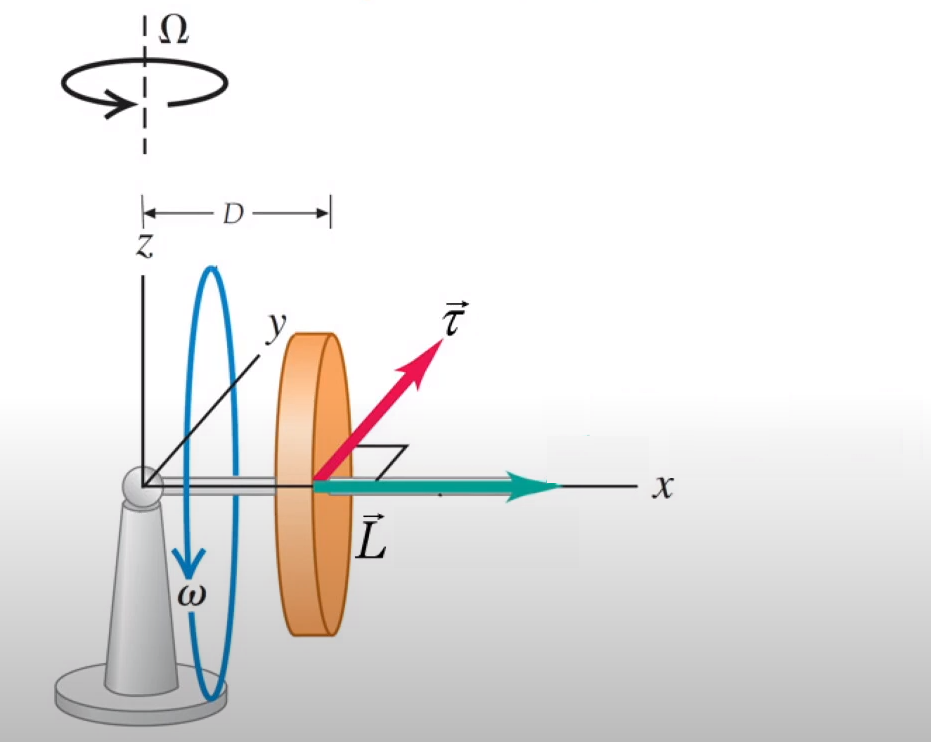
\includegraphics[width=\textwidth]{images/propriedades-giroscopio.png}
        \caption{Vetores que agem sobre o giroscópio}
    \end{subfigure}
\end{figure}

A partir dos diagramas acima, podemos realizar uma série de substituições de equações utilizando as equações básicas de rotação - como foi mostrado no vídeo dessa prática - para encontrar que a frequência da precessão $\Omega$ pode ser determinada pela seguinte equação:

\[ \Omega = \frac{MgD}{I \omega} \]

Com essa expressão em mãos podemos encontrar então o valor estimado da frequência de rotação do giroscópio $\Omega _e$.\\

Detalhe que para determinar \textit{I} haverá uma diferença nesse caso do giroscópio, pois diferente do Disco de Maxwell (tópico 2.1), não será possível desmontar a peça para pesar cada componente individualmente. Precisaremos calcular a massa da forma indireta, utilizando o valor da densidade do material que ela é feita.\\

Agora, como forma de comparação se soubermos o tempo que o giroscópio demora para fazer uma volta podemos calcular diretamente qual é a frequência de rotação $\Omega _d$ dada uma velocidade angular $\omega$ - que será medida utilizando um tacômetro. Esse valor $\Omega _d$ pode ser obtido pela simples relação:

\[ \Omega _d = \frac{2\pi}{\overline{t}} \]

% Onde $\overline{t}$ é o resultado da média aritmética dos

\newpage
\section{Resultados e discussão}

aaaaaaaaaa

\newpage
\section{Conclusões}

% =============== EXPERIMENTO 1 ===================== %

\subsection{Princípio de Arquimedes}

Maia

% =============== EXPERIMENTO 2 ===================== %

\subsection{Determinação do volume e da densidade de um sólido com
uma balança}

Maia

% =============== EXPERIMENTO 3 ===================== %

\subsection{Determinação do volume e da densidade de um sólido
utilizando um Areômetro de Nicholson}

Após realizarmos todos as etapas das aferições utilizando o Areômetro de Nicholson, pudemos encontrar uma densidade do sólido $\rho _s = 8,61 \pm 0,07 g/cm^3$ . Ao procurarmos em uma tabela de densidades, o valor que melhor representou a densidade do nosso sólido desconhecido, foi o material latão, que tem uma densidade tabelada de $\rho_l = 8,56 g/cm^3$ . \\

Comparamos os valores e confirmamos que os valores dessas duas densidades são \textbf{compatíveis}, checando que a densidade do latão está dentro do intervalo de incertezas da densidade do sólido - densidade experimental - como expresso no gráfico da figura 10.\\

Desse modo, pudemos comprovar a eficácia do nosso experimento, mostrando que o Areômetro de Nicholson é um método seguro de calcular volumes - e, consequentemente, densidades - de sólidos desconhecidos, porém, pode ser usado para o cálculo da densidade de líquidos desconhecidos (como feito por nós no experimento 4).\\

% =============== EXPERIMENTO 4 ===================== %

\subsection{Determinação da densidade de um líquido utilizando o
Areômetro de Nicholson}

Creppe


\newpage
\section{Bibliografia}

\begin{enumerate}
  \item SCHNEIDER, José F., AZEVEDO, Eduardo R. \textit{Laboratório de Física II: Livro de Práticas}. São Carlos, 2018.
  \item HALLIDAY, David; RESNICK, Robert; WALKER, Jearl. \textit{Fundamentos de Física - Volume 1}. 10a ed. Rio de Janeiro, RJ: LTC, 2018 vol 1;
  \item TIPLER, Paul A.; MOSCA, Gene, \textit{Física para Cientistas e Engenheiros - Volume 1}, 6a ed. Rio de Janeiro: LTC, 2012;
\end{enumerate}


\end{document}
